\textbf{Solución analítica del circuito:}

\textbf{Representación grafica: }


\begin{itemize}
	\item Considerando un periodo de muestreo de $ T_s = 1 $ y utilizando el método de discretización mediante
	diferencias finitas, encuentre la ecuación en diferencias asociada y resu´elvala utilizando el método de recurrencia. Compare los resultados gr´aficos de la versi´on de tiempo continuo y la de tiempo discreto para diferentes valores del periodo de muestreo (disminúyalo en un punto decimal hasta $T_s = 0,0001$).
\end{itemize}

\textbf{Comparación entre solución de tiempo discreto y aproximación con diferencias finitas para diferentes valores del tiempo de muestreo}

\begin{itemize}
	\item Obtenga la función de transferencia del sistema de tiempo continuo.
	\item Utilizando $ T_s = 1 $:
\end{itemize}

\textbf{A)} Obtenga la función de transferencia de tiempo discreto de la ecuación en diferencias que resultó en	el punto anterior.

\textbf{B)}  Obtenga la función de transferencia de tiempo discreto a partir de la función de transferencia de tiempo continuo del sistema utilizando un diferenciador discreto, ¿cómo son las funciones de transferencia obtenidas en este punto y el anterior? ¿qué puede concluir?


\begin{itemize}
	\item Grafique en una sola figura la respuesta al impulso del sistema de tiempo continuo, y las dos aproximaciones
	de tiempo discreto.
\end{itemize}

\textbf{Comparación de solución de tiempo contunuo y solución de tiempo discreto utilizando funciones de tranferencia}

\begin{itemize}
	\item Disminuya el tiempo de muestreo hasta obtener una aproximación adecuada de la respuesta del sistema
	y grafique la comparación. ¿Qu´e aproximación resultó mejor?
\end{itemize}

\textbf{Comparacion de solución de tiempo continuo y solución de tiempo discreto utilizando funciones de tranferencia para diferentes valores de tiempo de muestreo }

{\Large Control discreto de un sistema de tiempo continuo.}

Considere un sistema lineal e invariante en el tiempo representado por la siguiente función de transferencia

\begin{equation*}
	G(s)=\frac{1}{s(s+3)}
\end{equation*}

\begin{itemize}
	\item Determine la estabilidad del sistema.
Para poder determinar la estabilidad del sistema, vamos a ver con MATLAB en donde se encuentran sus Polos. Para ello vamos a escribir los siguientes comandos.\\
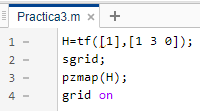
\includegraphics[scale=1]{cod1.png}\\
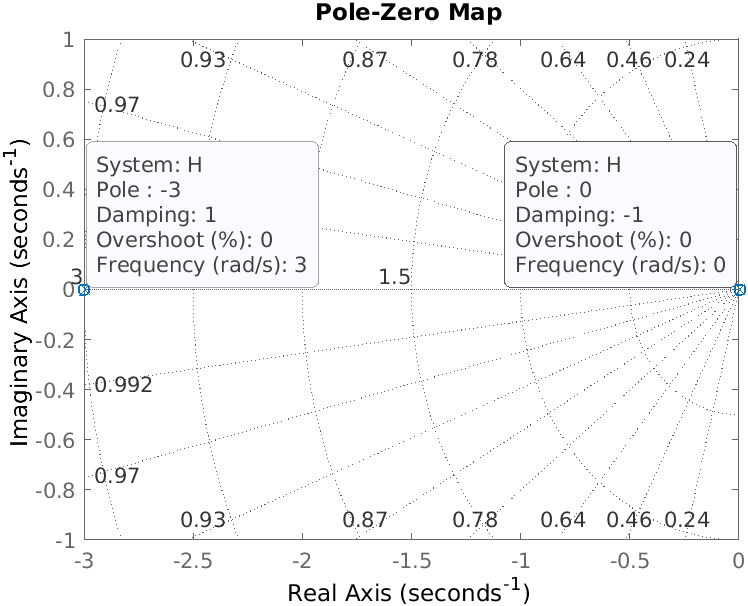
\includegraphics[scale=1]{G1.png}\\ \\
Como se puede ver un polo esta en s=-3, pero el otro polo esta en s=0, por lo que no podemos decir si el sistema es estable o no. Ya que para que un sistema sea estable TODOS sus polos deben de estar en la parte izquierda del plano S. Por lo que primero veremos su respuesta al escalón para así poder determinar si el sistema es estable o no.

	\item Utilizando el software especializado de su preferencia, determine la respuesta al escalón del sistema y describa como es su comportamiento.
Para determinar la respuesta al escalón del sistema vamos a agregar el siguiente comando al código anterior: step(H,'-')\\
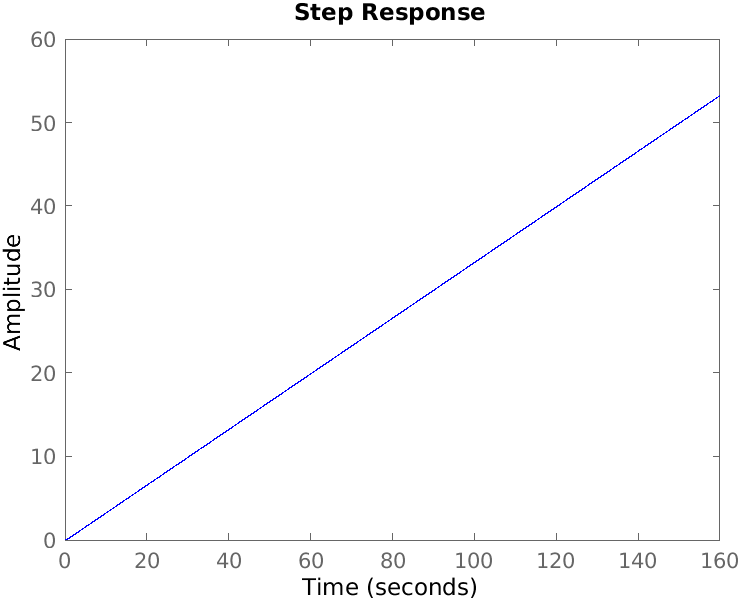
\includegraphics[scale=1]{G2.png} \\ \\
Al analizar esta gráfica podemos ver que no tiene fin, en otras palabras la gráfica no tiene limite, ya que solamente es creciente conforme va avanzando en el eje X positivo. Por lo que podemos concluir a la pregunta anterior que NO es estable el sistema.

\end{itemize}

\begin{figure}[H]
	\centering
	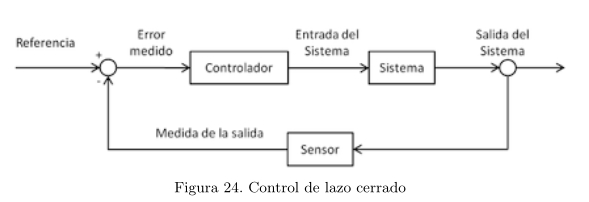
\includegraphics[scale=0.7]{img2/fig24}
	\label{fig:fig24}
\end{figure}

\textbf{Respuesta al escalón del sistema a controlar}

\begin{itemize}
	\item Cuando se desea cambiar el comportamiento de un sistema se debe implementar un controlador de lazo
	cerrado, el cual compara la se˜nal de salida del sistema con la se˜nal de referencia y con base en esta se˜nal
	de error calcula la entrada del sistema para que se obtenga el comportamiento deseado, de acuerdo con
	el diagrama de bloques mostrado en Figura 24. El modo m´as simple de control consiste en el control
	proporcional, el cual realimenta un término proporcional del error de salida, es decir,
\end{itemize}

\begin{equation*}
	u_c=K(r-y)
\end{equation*}

La conexión de la Figura 24 se denomina conexión en retroalimentación negativa, y es posible determinar la función de transferencia correspondiente mediante software especializado, para lo cual se deben definir
previamente las funciones de transferencia del controlador, del sistema y del sensor. Considerando la función de transferencia del sistema, la del controlador como C(s) = K y la del sensor H(s) = 1, determine
la función de transferencia de lazo cerrado Gc(s) correspondiente. ¿Cómo son los polos del sistema? ¿Qué puede decir de la estabilidad del mismo?
$$E(s)=R(s)-Y(s)$$
Donde: E(s) es el error medido, R(s) es la referencia y Y(s) es la salida.
$$H(s)=frac{Y(s)}{X(s)}$$
$$Y(s)=H(s)KX(s)$$
Si E(s)=X(s):
$$Y(s)=H(s)KE(s)$$
$$Y(s)=\frac{1}{s(s+3)}KE(s)$$
$$Y(s)=\frac{KE(s)}{s(s+3)}$$
$$E(s)=\frac{Y(s)(s(s+3))}{k}$$
Si $E(s)=R(s)-Y(s)$
$$R(s)-Y(s)=\frac{Y(s)(s(s+3))}{k}$$
$$KR(s)-KY(s)=Y(s)(s(s+3))$$
$$KR(s)=Y(s)(s(s+3)+K)$$
$$G_{c}(s)=\frac{Y(s)}{R(s)}=\frac{K}{s(s+3)+K}$$
Función de transferencia de lazo cerrado:
$$G_{c}(s)=\frac{Y(s)}{R(s)}=\frac{K}{(s(s+3)+K)}$$	
Si k=1:
$$G(s)=\frac{1}{(s(s+3)+1)}$$	
$$G(s)=\frac{1}{s^{2}+3s+1}$$	
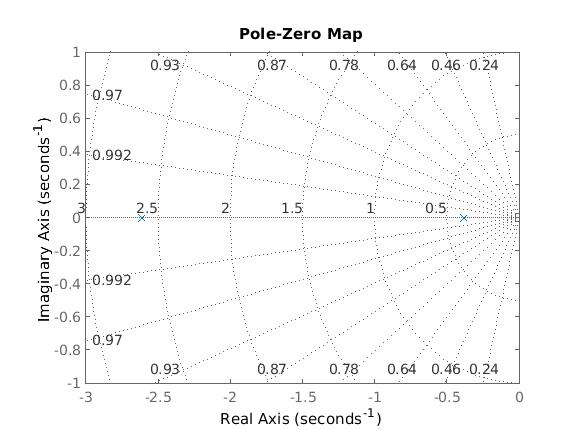
\includegraphics[scale=0.5]{G3.jpg}\\ 
Polos: $P_{1}=-2.618$ y $P_{2}=-0.382$. Por lo tanto es estable el sistema.\\\\
Respuesta al escalón del sistema:\\
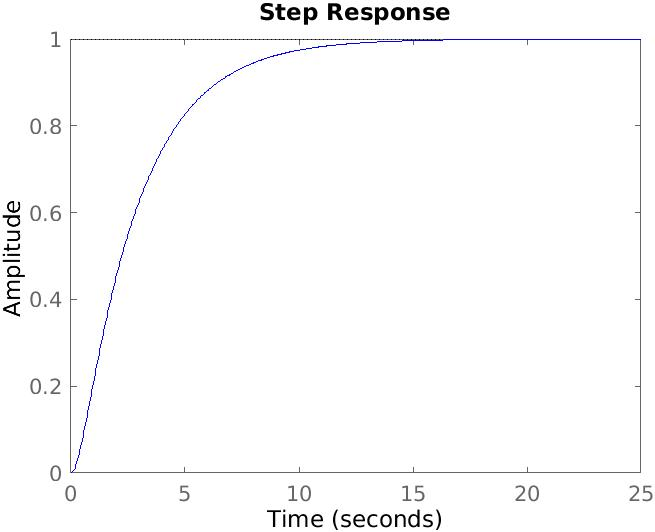
\includegraphics[scale=0.4]{G5.jpg}\\
Si k=-10:
$$G(s)=\frac{-10}{(s(s+3)-10)}$$	
$$G(s)=\frac{-10}{s^{2}+3s-10}$$
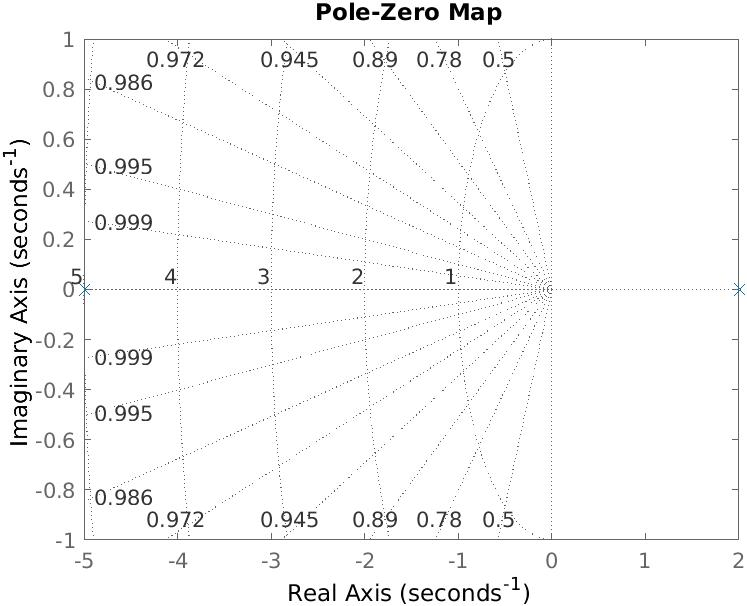
\includegraphics[scale=0.36]{G4.jpg}\\ 	
Polos: $P_{1}=-5$ y $P_{2}=2$. Por lo tanto es inestable el sistema.\\\\
Respuesta al escalón del sistema:\\
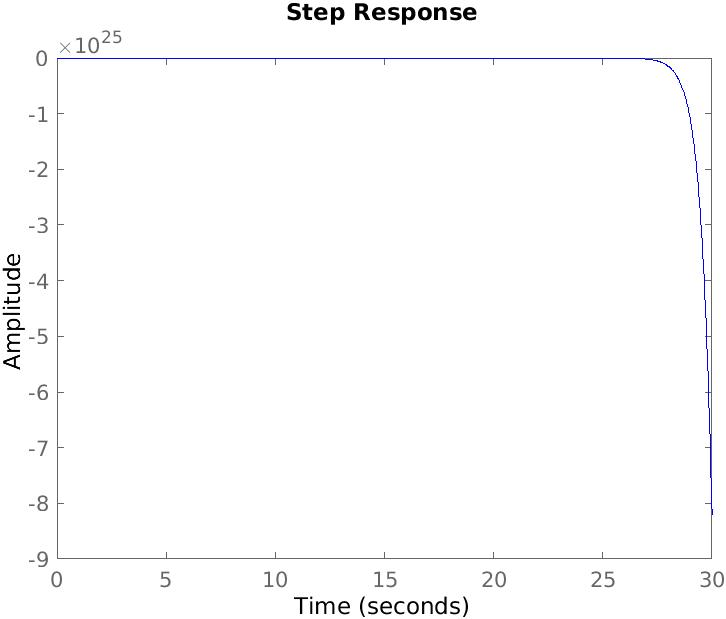
\includegraphics[scale=0.36]{G6.jpg}\\
¿Cómo son los polos del sistema? Dependiendo del valor de K los polos del sistema van a variar. Por lo que pueden volver estable o inestable al sistema.\\
¿Qué puede decir de la estabilidad del mismo? Lo que podemos ver con estos dos valores de K, es que dependiendo de su valor, se modificará la entrada del sistema, volviéndose estable o inestable el sistema.

\begin{itemize}
	\item A partir de las funciones de transferencia de lazo abierto y de lazo cerrado en tiempo continuo obtenga las versiones de tiempo discreto. Realice lo anterior utilizando los procedimientos presentados en la
	Introducción Teórica y el software especializado de su elección. Reporte sus resultados a continuación.
\end{itemize}

\textbf{Respuesta al escalón del sistema con control}

\begin{itemize}
	\item Determine los polos de lazo abierto y de lazo cerrado de tiempo discreto y caracterice la estabilidad de
	cada uno de estos. Determine la respuesta al escalón de ambos sistemas utilizando software especializado.
	Escriba sus resultados a continuación y las gráficas obtenidas en los espacios correspondientes.
\end{itemize}

\textbf{Respuesta al escalón del sistema en tiempo discreto}

\textbf{Respuesta al escalón del sistema de control en tiempo discreto}